\usepackage{graphicx}
\graphicspath{ {img/} }

\chapter{Funzioni a due variabili}

\section{Generalità}

\section{Limiti}

Diciamo che $\lim_{(x,y)\to(x_0,y_0)} f(x,y) = L$ se e solo se fissato un numero reale positivo $\epsilon>0$ esiste un $\gamma>0$ tale che se $(x,y)$ appartengono all'intorno bucato di $(x_0,y_0)$ di raggio $\gamma$ allora $|f(x,y)-L|<\epsilon$

\section{Continuità}

Una funzione $f(x,y)$ si dice continua in un punto $(x_0,y_0)$ se:

\begin{itemize}
\item E' definita in $(x_0,y_0)$
\item Esiste il limite $\lim_{(x,y)\to(x_0,y_0)} f(x,y)$ ed è uguale a $f(x_0,y_0)$
\end{itemize}

Quindi non è detto che se esiste il limite di una funzione in un punto allora la funzione è definita in quel punto.

\section{Derivabilità}

\subsection{Derivata in $R$}

$$f'(x_0)=\lim_{h\to 0}\frac{f(x_0+h)-f(x_0)}{h}$$

\subsection{Derivate Parziali}

Calcolate solo rispetto all'asse $x$ o all'asse $y$.
 
\begin{figure}[h]
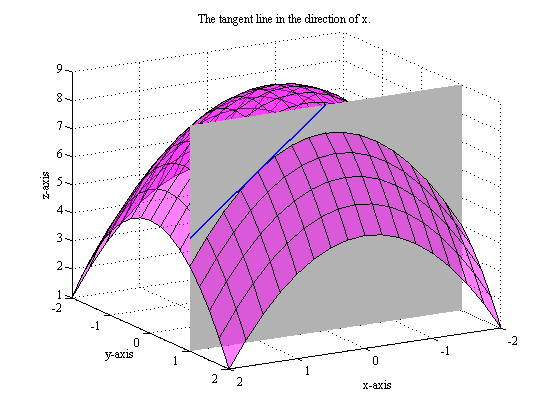
\includegraphics[width=\textwidth]{diff_partial.png}
\end{figure}

$$
f_x(x_0,y_0) = \lim_{h\to 0} \frac{f(x_0+h,y_0)-f(x_0,y_0)}{h}
$$

$$
f_y(x_0,y_0) = \lim_{k\to 0} \frac{f(x_0,y_0+k)-f(x_0,y_0)}{k}
$$

\subsection{Derivata direzionale}

Calcolata rispetto ad una qualsiasi retta/direzione.

Fissato un qualunque vettore $V=(v_1,v_2)$ non nullo posso provare a calcolare:

$$
f_v(x_0,y_0) = \lim_{h\to 0} \frac{f(x_0+v_1h,y_0+v_2h)-f(x_0,y_0)}{h}
$$

La derivata direzionale si puo' anche definire rispetto ai soli versori, cioè i vettori che hanno norma 1, visto che anche solo con questi si possono \textit{identificare} tutte le direzioni.

La derivata direzionale è anche uguale a $$\nable f(x_0,y_0)\cdot V$$

\subsection{Sviluppo di Taylor}

$$f(x,y) = f(x_0,y_0)-f_x(x_0,y_0)(x-x_0)+f_y(x_0,y_0)(y-y_0)+ \
\frac{1}{2} [f_{xx}(x_0,y_0)(x-x_0)^2+2f_{xy}(x_0,y_0)(x-x_0)(y-y_0)+f_{yy}(x_0,y_0)(y-y0)^2]+ \
o((x-x_0)^2+(y-y_0)^2)
$$

\section{Differenziabilità}

\subsection{Differenziabilità in $R$}

Una funzione $f$ è differenziabile in $x_0$ se esiste un numero $\alpha \in R$ tale che:

$$f(x_0+h)=f(x_0)+\alpha h + o(h)$$

per $h \to 0$.
 
\subsection{Generalità}

Si dice che la funzione $f(x,y)$ è differenziabile in $(x_0,y0)$ se vale che: 
$$
\lim_{(h,k)\to (0,0)} \frac{f(x_0+h,y_0+k) - f(x_0,y_0) - h A - k B}{\sqrt{h^2+k^2}} = 0
$$
dove $A=f_x(x_0,y_0)$ e $B=f_y(x_0,y_0)$

\subsection{Condizioni esistenza}

Per essere differenziabile una funzione deve essere continua e deve ammettere derivate parziali in $(a,b)$ lungo ogni direzione $V \in R^2$ (e quindi anche le derivate parziali).

\subsection{Gradiente}

Chiamiamo $\nabla f(x_0,y_0)$ il gradiente della funzione $f$ calcolato in $(x_0,y_0)$. 

$$ \nabla f(x_0,y_0) = (f_x(x_0,y_0),f_y(x_0,y_0))$$

Il vettore gradiente calcolato in un punto è anche detto \textbf{differenziale} della funzione in quel punto.

\subsubsection{Interpretazione geometrica}

\textbf{Per quali versori di $V$ la derivata direzionale risulta Massima o Minima?}

$$
f_V(x_0)  = |\nabla f(x_0)| \cdot |V| \cdot \cos(\theta)
$$

Visto che stiamo trattando versori allora $|V|=1$.

Quindi è la derivata direzionale è massima per $\cos(\theta)=1 \rightarrow \theta=0$

Quindi è la derivata direzionale è minima per $\cos(\theta)=0 \rightarrow \theta=\pi$

La direzione del gradiente calcolato in un punto indica la retta seguendo la quale si trova il massimo incremento della funzione $f$ nell'intorno del punto in cui è calcolato.

\subsection{Differenziale}

\subsubsection{Generalità}

Se le derivate prime esistono, possiamo definire il differenziale: il differenziale di una funzione quantifica la variazione infinitesimale della funzione rispetto ad una variabile indipendente.


\section{Punti di massimo e di minimo}

\subsection{Matrice Jacobiana}

La matrice jacobiana di una funzione è la matrice i cui elementi sono le derivate parziali prime della funzione.

La sua importanza è legata al fatto che, nel caso la funzione sia differenziabile, la jacobiana rappresenta la migliore approssimazione lineare della funzione vicino a un punto dato.


Sia $\mathbf{f}: U \rightarrow \mathbb R^m$ una funzione definita su un insieme aperto $U$ dello spazio euclideo  $\mathbb R^n$ . La matrice jacobiana della funzione $J {\mathbf f}$ in $\mathbf x = (x_1, \dots, x_n)$ è la matrice delle derivate parziali prime della funzione calcolate in $\mathbf x$:

$$J \, \mathbf f = \begin{bmatrix} \dfrac{\partial f_1}{\partial x_1} & \cdots & \dfrac{\partial f_1}{\partial x_n} \\ \vdots & \ddots & \vdots \\ \dfrac{\partial f_m}{\partial x_1} & \cdots & \dfrac{\partial f_m}{\partial x_n}  \end{bmatrix}\qquad \operatorname (J \, \mathbf f)_{ij} = \frac{\partial f_i (\mathbf {x})}{\partial x_j} $$


\section{Integrali doppi}

\section{Generalità}

$$\iint_A f(x,y) \dif x \dif y$$

$A$ è l'insieme (zona) di integrazione, \textbf{sottoinsieme limitato} del piano.

$f(x,y) A\to R$ è una funzione limitata. Esiste cioè un $M$ tale che $|f(x,y) \leq M \forall (x,y) \in A$.

\section{Significato geometrico}

\subsection{In $R$}

$$\int_a^b f(x) \dif x$$

L'integrale + l'area con segno della parte di piano sottesa alla funzione $f(x)$.

\subsection{In $R^2$}

$$\iint_A f(x,y) \dif x \dif y$$

se $f(x,y) \ge 0$ allora è il volume della parte di spazio compresa tra il piano $xy$ ed il grafico di $f(x,y)$, limitata dalle \textit{pareti verticali} che si proiettano sul bordo di $A$.

se $f(x,y)$ ha segno qualunque le parti sotto il piano $xy$ contano con il segno $-$.

\section{Come si definiscono}

\subsection{Funzione costante su un rettangolo}

$A= [a,b] \bigtimes [c,d]$

Cioè $A$ è un rettangolo delimitato dai lati $ab$ e$cd$.

$f(x,y) = \lambda$, cioè una costante.

Quindi l'integrale è semplicemente $$\lamda \cdot (b-a) \cdot (d-c)$$ volume con segno del parallelepipedo.
 
\subsection{Funzioni costanti su più rettangoli}

$A$ è un' unione disgiunta di rettangoli.

(Come tanti grattacieli uno vicino all'altro).

$f(x,y)$ è costante all'interno di un rettangolo, ma puo' variare da rettangolo a rettangolo.

$f(x,y) = \lamba_i \forall (x,y) \in R_i$.

Quindi l'integrale é $$\sum_{i=1}^{n} \lambda_i * \text{Area}(R_i)$$.

\subsection{Funzione non costante su un rettangolo}

$D$ è un rettangolo chiuso, con lati paralleli agli assi. 

$f(x,y)$ è una funzione (costante o no) definita sul dominio $D$.

Supponiamo che D varia tra $a$ e $b$ sull'asse $x$ e tra $c$ e $d$ sull'asse $y$.

Possiamo quindi partizionare il dominio in dei rettangoli più piccoli, individuando dei punti in questo modo:

$$a = x_0 < x_1 < \ldots < x_{m-1} < x_m = b$$


$$c = y_0 < y_1 < \ldots < y_{n-1} < y_n = d$$

In sostanza si individuano $m \cdot n$ rettangoli $R_{ij}$..

L'area di ogni rettangolo è $$\delta A_{ij} = \delta x_i \delta y_1$$

La lunghezza della iagonale è 
$$\sqrt{(\delta x_i)^2+(\delta y_i)^2}$$

Scelto un punto arbitrario $(x_{ij},y_{ij})$ in ciascuno dei rettangoli individuiamo la somma di Riemann:
$$R(f,P_{artizione}) = \sum^m_{i=1} \sum^n_{j=1} f(x_{ij},y_{ij}) \delta A_{ij}$$

In sostanza base per altezza di un parallelepipedo.

Facendo il limite 
$$\lim_{n,m \to infty} R(f,P_{artizione})$$ otteniamo l'integrale doppio di $f$ su $D$, cioè il volume sopra $D$ e sotto il grafico di $f$.


\section{Funzione integrabile}

\begin{definition}
Si dice che $f$ è integrabile sul rettangolo $D$ e che ha integrale doppio $$I = \iint_D f(x,y) \diff A$$
se, per ogni numero positivo $\epsilon$, esiste un numero $\gamma(\epsilon)$ tale  che $$R(f,P)-I<\epsilon$$ vale per ogni $P$ di $D$ tale che $|P|<\gamma$ e per tutte le scelte di punti $(x_{ij},y_{ij})$. 
\end{definition}

\begin{property}
Se una funzione è continua su $D$ allora è integrabile su $D$. Ma non è detto che se è integrabile allora è continua.
\end{property}

\section{Integrali doppi su domini generali}

Potrebbe anche essere necessario calcolare un integrale su un dominio $D$ che non è un rettangolo ma un area qualunque del piano. 

